\documentclass[a4paper,10pt]{article}


%%++++++++++++++++++++++++++++++++++++++++++++++++++++++++++++++++++++++++++++++
%%  Packages
\usepackage[english]{babel} 			% Langue
\usepackage[utf8]{inputenc}											% Encodage
\usepackage[T1]{fontenc}											  % Requis

\usepackage[pdftex]{graphicx}										% Images 
\usepackage{fancyhdr}												% Spécifier Entête et pieds.
\usepackage[margin=2.5cm]{geometry}

\usepackage{url}													% URL 
\usepackage{hyperref}
\usepackage{verbatim}												% Texte entre 	\begin{verbatim}  \end{verbatim} ne sera pas interprété
\usepackage{listliketab}											% List spéciale, notament comme tableau
\usepackage{longtable}
\usepackage{booktabs}												% Permet de faire des tableau plus avec des traits
% Exemple:
%\begin{tabular}{llr}
%\toprule
%\multicolumn{2}{c}{Item} \\
%\cmidrule(r){1-2}
%Animal & Description & Price (\$) \\
%\midrule
%Gnat  & per gram & 13.65 \\
%      & each     &  0.01 \\
%\bottomrule
%\end{tabular}

\usepackage{color}		
%% \definecolor{orange}{RGB}{255,127,0} http://en.wikibooks.org/wiki/LaTeX/Colors

\usepackage{tabularx}											% Tableau streatching 
\usepackage{colortbl}											% Permet des tableaux exotiquement colorier 
\usepackage{wrapfig}											% Permet d'alligner une figure à guache ou à droite
%\begin{wrapfigure}{r}{40mm}
%  \begin{center}
%    \includegraphics{toucan.eps}
%  \end{center}
%  \caption{The Toucan}
%\end{wrapfigure}
\usepackage{rotating}
\usepackage{amsmath}
\usepackage{subfig}
\usepackage{pdfpages}										% inclus pdf http://www-hep2.fzu.cz/tex/texmf-dist/doc/latex/pdfpages/pdf-ex.pdf
\usepackage[subfigure]{tocloft}
%\begin{figure}[htp]
%  \begin{center}
%    \subfigure[Original image]{\label{fig:edge-a}\includegraphics[scale=0.75]{toucan.eps}}
%    \subfigure[After Laplace edge detection]{\label{fig:edge-b}\includegraphics[scale=0.75]{laplace_toucan.eps}} \\
%    \subfigure[After Sobel edge detection]{\label{fig:edge-c}\includegraphics[scale=0.75]{sobel_toucan.eps}}
%  \end{center}
%  \caption{Various edge detection algorithms}
%  \label{fig:edge}
%\end{figure}
\usepackage[table]{xcolor}								
\usepackage{url}	
%\usepackage{lscape} 								%% Texte en landspcae
%\begin{landscape}
%notre texte
%\end{landscape}

%%++++++++++++++++++++++++++++++++++++++++++++++++++++++++++++++++++++++++++++++
%%  macros
\newcommand{\todo}[1]{\colorbox{red}{\color{white}:TODO:}#1}



\usepackage{listings}
%\lstset{
%language=C,
%basicstyle=\small\sffamily,
%numbers=left,
%numberstyle=\tiny,
%frame=tb,
%columns=fullflexible,
%showstringspaces=false
%}
\lstset{language=C,captionpos=b,tabsize=3,frame=lines,keywordstyle=\color{blue},commentstyle=\color{darkgreen},stringstyle=\color{red},numbers=left,numberstyle=\tiny,numbersep=5pt,breaklines=true,showstringspaces=false,basicstyle=\footnotesize,emph={label}}

%%%%%%%%%%%%%%%%%%%%%%%%
%%  Design
%%%%%%%%%%%%%%%%%%%%%%%%%%
%%
%%  Pren1 Schlussdokument
%%  Kopf und Fusszeilen
%%  CT
%%
%%%%%%%%%%%%%%%%%%%%%%%%

\pagestyle{fancy}
  \renewcommand\headrulewidth{0.4pt}
  \fancyhf{}
  \setlength{\headheight}{35.60004pt}
%  \addtolength{\texthight}{-2*\headheight}
  \lhead{
    \protect
\includegraphics[height=32pt]{./images/model/eifr-logo.jpg}
  }
  \rhead{
    Microprocessors 3 - Intel Assembler\\
   Jonathan Stoppani et Elias Medawar\\
  }
  \cfoot{
    \thepage
  }
\fancypagestyle{plain}{
  \renewcommand\headrulewidth{0.4pt}
  \fancyhf{}
  %\addtolength{\headheight}{\baselineskip}
  \lhead{
    \protect
\includegraphics[height=32pt]{./images/model/eifr-logo.jpg}
  }
  \rhead{
  Microprocessors 3 - Intel Assembler\\
     Jonathan Stoppani et Elias Medawar\\
  }
  \cfoot{
  }
}
\fancypagestyle{empty}{
  \renewcommand\headrulewidth{0pt}
  \fancyhf{}
  %\addtolength{\headheight}{\baselineskip}
  \lhead{
  }
  \cfoot{
  }
}

\begin{document}
	\begin{titlepage}
	
	%\sffamily

		
	\addtolength{\leftskip}{-1cm}\addtolength{\rightskip}{-3.5cm}
	%\sffamily
	\vfill
	
	\hspace{0.10cm}	
\includegraphics{./images/model/eifr-logo.jpg} 

	\vfill
	\hspace{8.99cm}\Huge Microprocessors  3 
	
	\hspace{9.08cm}\LARGE Report lab 3 : Pipeline
	      
	\vfill
	\Large
	
	\hspace{9.08cm}  Jonathan Stoppani et Elias Medawar
	
	\vfill
	\hspace{9.08cm}\normalsize Version:  \today
	\vfill
	\thispagestyle{empty}
	\clearpage

\end{titlepage}

	
	%%%%%%%%%%%%%%%%%%%%%%%%
%%
%%  Pren1 Schlussdokument
%%  Kopf und Fusszeilen
%%  CT
%%
%%%%%%%%%%%%%%%%%%%%%%%%

\pagestyle{fancy}
  \renewcommand\headrulewidth{0.4pt}
  \fancyhf{}
  \setlength{\headheight}{35.60004pt}
%  \addtolength{\texthight}{-2*\headheight}
  \lhead{
    \protect
\includegraphics[height=32pt]{./images/model/eifr-logo.jpg}
  }
  \rhead{
    Microprocessors 3 - Intel Assembler\\
   Jonathan Stoppani et Elias Medawar\\
  }
  \cfoot{
    \thepage
  }
\fancypagestyle{plain}{
  \renewcommand\headrulewidth{0.4pt}
  \fancyhf{}
  %\addtolength{\headheight}{\baselineskip}
  \lhead{
    \protect
\includegraphics[height=32pt]{./images/model/eifr-logo.jpg}
  }
  \rhead{
  Microprocessors 3 - Intel Assembler\\
     Jonathan Stoppani et Elias Medawar\\
  }
  \cfoot{
  }
}
\fancypagestyle{empty}{
  \renewcommand\headrulewidth{0pt}
  \fancyhf{}
  %\addtolength{\headheight}{\baselineskip}
  \lhead{
  }
  \cfoot{
  }
}
	
	\section{ Find the password used by the programm}
		\begin{enumerate}
		\item Run the program and analyse the basic functionality
		\subitem The program display Enter password 
		\subitem We enter the password
		\subitem The program write Bad password. 
		\item use the command strings to analyse if there is some relevant string that can be a password. 
		\subitem To many strings we can not exploit this method
		\item objdump -d password\_1
		\subitem find main section, found a call for strcomp (string compare)
		\subitem Just before the call of strcomp will move on the stack 2 arg .
		\subitem One arg is the entered password and the second arg is a pointer(0x080497d0).
		\item use ddd to find the value of the pointer (display 0x080497d0)
		\subitem we found the value 0x08048614
		\item use ddd to display the value at address 0x08048614
		\subitem we found the password : scanf
		\end{enumerate}
			\begin{center}
						 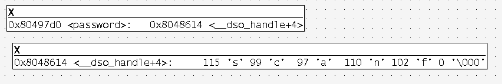
\includegraphics[width=0.8\textwidth]{./images/withDebug}
				\end{center}
		\subsection{Alternative}
		\begin{enumerate}
			\item use readelf -x <24(data)> to read the fixed values
			\subitem we found the pointer to the value in the rodata section
			\item use readelf -x <15(rodata)> to read the value of the password.
			\subitem we found the password: scanf
		\end{enumerate}
		
		\section{When the password is found, delete the symbols with the command strip  and use ddd without symbols}
			\begin{enumerate}
				\item strip password\_1
				\item open the program with ddd
				\item with the console add a breakpoint in the main section(break @)
				\item with the console run the program and display the values of the pointer 
				\end{enumerate}
					\begin{center}
										 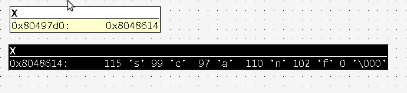
\includegraphics[width=0.8\textwidth]{./images/withoutDebug}
					\end{center}
\end{document}